% !TeX root = ../main.tex
% Add the above to each Chapter to make compiling the PDF easier in some editors.

\chapter{Introduction}\label{Chapter:introduction}

This chapter presents the most relevant previous research contributions to the studied snake robot locomotion method and the hybrid position/force control method. Furthermore, the scope of the project and its contributions are summarized. The simplification and limitations, as well as the snake robot model description can be found in this chapter as well. Lastly, the structure of the report is described.

\section{Previous work}

The department of engineering cybernetics at the Norwegian University of Science and Technology (NTNU) has made significant contributions to the field of snake robot control, related to both aquatic snake-like propulsion and efficient snake robot locomotion on flat surfaces \cite{StavdahlNote}.

Some common modes of snake robot locomotion on flat surfaces are lateral undulation, concertina locomotion and sidewinding. Lateral undulation and sidewinding are dependent on ground friction for the snake robot to propel itself forward, whereas concertina locomotion utilizes walls or narrow spaces that the snake robot can anchor itself against and push itself forward. Terrestrial snake robot locomotion can also be achieved by utilizing more irregular obstacles in the terrain, such as rocks. Directional compliance, proposed by Wang et al. \cite{wang2020directional} in 2020, is a novel method that adapts the snake robot shape to obstacles it collides with in the environment and use them to enhance the existing propulsion mode and avoid getting jammed between obstacles.

\textit{Obstacle Aided Locomotion (OAL)} is on the other hand a method that uses obstacles as the main part of the locomotion strategy and always seeks to find the obstacles that can profit the propulsion the most. The idea of this method, which was introduced by Transeth et al. \cite{transeth2008snake} in 2008, is that the snake robot pushes against obstacles in order to propel itself forward along a predefined path. The principle is comparable to lateral undulation, where ground friction is used instead of obstacles to push against. It is thus possible to say that OAL is a very discrete special case of lateral undulation. For this reason it is believed that solutions and findings regarding OAL can later be used to profit and optimize snake robot locomotion gaits like lateral undulation.

%This method relies on the force sensor feedback received at any point in time in order to calculate the desired shape of the robot. \hl{skriv bedre takk}

In OAL it is desired to control the force against obstacles and shape of the robot independently. Thus, Stavdahl \cite{StavdahlNote} proposed a combination of OAL and \textit{Hybrid Position/Force Control (HPFC)}, leading to the term \textit{Hybrid Obstacle Aided Locomotion (HOAL)}. Klafstad \cite{TorjusOppg} summarized the theory around this concept in 2018, and it was further researched and tested by the author in her previous project work \cite{AtussaProsjektoppgp} in 2019, both with emphasis on the HPFC method introduced by West and Asada \cite{west1985method} in 1985. This method was developed after the concept was first introduced by Raibert et al. in 1981 \cite{raibert1981hybrid}, and aims at controlling constrained robot manipulators based on kinematic projections of the motion and force such that these variables comply with both the allowable and desired behaviour of the snake robot. Yoshikawa \cite{yoshikawa1987dynamic} advanced the method in 1987 by including the dynamics of the robot in the control calculations.

The research of HPFC has mainly been focused on the control of traditional robot manipulators. Nansai et al. \cite{nansai2016dynamic} applied HPFC on snake robots with wheels in 2016. The wheels restrict direct sideways movement of the robot and can therefore be considered as obstacles on the sides of the snake robot. The HPFC was however not applied for the locomotion of the robot, but for a typical robot manipulator task the snake robot was set to execute. A lot of work still remains when it comes to combining snake robot OAL with HPFC. Because the behaviour of the snake robot is driven by its dynamics, the research is now continued to explore the dynamic HPFC method in light of HOAL.



\section{Scope of the project}

\subsection{Thesis assignment interpretation}

The detailed assignment for this thesis is provided in the very beginning of the report. The author's perception is that the main focus lies on mathematically adapting the dynamic HPFC method of Yoshikawa \cite{yoshikawa1987dynamic} to the snake robot case with special attention to the snake robot force and position spaces. A control structure should then be designed and implemented in a carefully selected simulator to conduct experiments that help evaluate important aspects of the developed method. A discussion of how the dynamic HPFC method can be used to achieve HOAL should also be carried out.
%and the limitations of the HOAL problem in light of which tasks can be realized based on the position and force spaces of the robot.

%This section thoroughly describes the authors interpretation of the different tasks.

%It is understood that some background theory on existing terrestrial locomotion strategies should be provided. It should then be discussed  whether or not they can be combined with the dynamic HPFC method.
%Furthermore, the dynamic HPFC method of Yoshikawa \cite{yoshikawa1987dynamic} is to be mathematically adapted to snake robots. Special attention should here be payed to the modifications that have to be made as a result of the differences between snake robots and traditional robot manipulators. A discussion should be carried out of how the dynamic HPFC method can be used to achieve OAL, and the limitations of the HOAL problem in light of which tasks can be realized based on the position and force spaces of the robot. Furthermore, some sufficient and necessary conditions for propulsion are to be suggested.

%Lastly, a control structure to test the dynamic HPFC algorithm should be designed. A suitable simulator needs to be found and evaluated for this purpose. The performance of the dynamic HPFC method on snake robots should be tested.




\subsection{Contributions}

The most significant contributions from this project lie in the mathematical adaptation of the dynamic HPFC method to snake robots intended to perform HOAL. An analysis of further control requirements and associated improvements and modifications to the method are also provided. Furthermore, a discussion is carried out of the requirements to the snake robot itself and its configuration relative to the obstacles it is in contact with.

The developed snake robot model and dynamic HPFC method have been implemented and tested in a simulation environment after a simulator was thoroughly chosen. Furthermore, a review of this simulator and a comparison to other corresponding simulators is provided. A guiding description of the simulator structure and how it generally can be utilized is also prepared and to be found in the report. Lastly, the findings have been discussed in light of HOAL and improvements to the dynamic HPFC method and control structure are proposed.


\section{Model specifications} \label{ch:model_specs}

This section presents the physical aspects of the snake robot model used throughout the report. The model has three main parts, namely the environment, the snake robot and the obstacles. The value of all variables needed to express the model and control goals are assumed known at all times. Further simplifications and assumptions are presented below. The parts \textit{Assumptions} and \textit{Further model description} are taken from the previous work of the author \cite{AtussaProsjektoppgp}, but some of the assumptions are modified to conform with the current project.

\subsection{Simplifications}

Snake robots performing OAL are typically in contact with several obstacles at a time and it is thus desired to control the snake robot at several contact points simultaneously. A higher number of joints and therefore actuators are beneficial for execution of this kind of control. However, in order to reduce the dimensions of the dynamic and kinematic calculations, the snake robot model used for testing consists of six links and five joints, which has limited the possible test variations.

The computed snake robot model is designed for a very specific scenario in which it is assumed that there are three contacts between a predefined set of snake robot links and obstacles at all times. Consequently, all movement of the snake robot can only be performed in the bounds of this assumption, meaning at most one link length displacement.

Another simplification made in the mathematical model is that the snake robot and obstacles are assumed to be 2D bodies, although they have 3D properties in the simulator. However, since all movement and control happens in the 2D plane it is not considered to have been a very evident deficiency.

The collisions between the snake robot and obstacles are not modeled because it is assumed that the contact is maintained at all times. However, small collisions are experienced by the simulator as a result of a sensitive force sensor and the contact point on a link moving within the range of the link.


\subsection{Assumptions}\label{seq:assumptions}

Assumptions 1-6 are taken from Stavdahl \cite{StavdahlNote}, whilst assumptions 7-9 are specific for this project.

\begin{enumerate}
    \item All parts of the model are assumed to be rigid.
    \item The robot has $n$ joints and all links have length $l$ and mass $m$.
    \item Only flat, 2-dimensional cases are considered.
    \item The robot has no lateral extension.
    \item There is no friction. 
    \item Obstacles have no spatial extent, only a static position in the plane.
    %\item During an impact with an obstacle, the configuration of the snake robot, $\mathbf{q}$, remains unaltered while the velocity, $\mathbf{\dot{q}}$, will generally experience a jump.
    \item Any link is in contact with at most one obstacle at the time.
    \item The robot is in touch with obstacles in its start configuration.
    \item Contact between a link and an obstacle is maintained.
\end{enumerate}

%----------------------------------------------------------------------------------
%----------------------------------------------------------------------------------

\subsection{Further model description}

\subsubsection{The snake robot}
The snake robot itself is modeled as a simple planar robot manipulator with links and joints. The main difference between the snake robot and a classic robot manipulator is the property that the snake robot is not physically attached to any fixed point in the world. This frees one constraint. However, it is still relevant to express the position of the first link of the snake, also denoted as the tail. This is performed by introducing three virtual joints to the model; two translational and one rotational joint. These joints are not controllable and merely for describing the kinematics, dynamics and constraints. The model of the snake robot is visualized in Figure \ref{fig:2_kin}, where physical robot links are blue and the virtual ones are green.

\begin{figure}
    \centering
    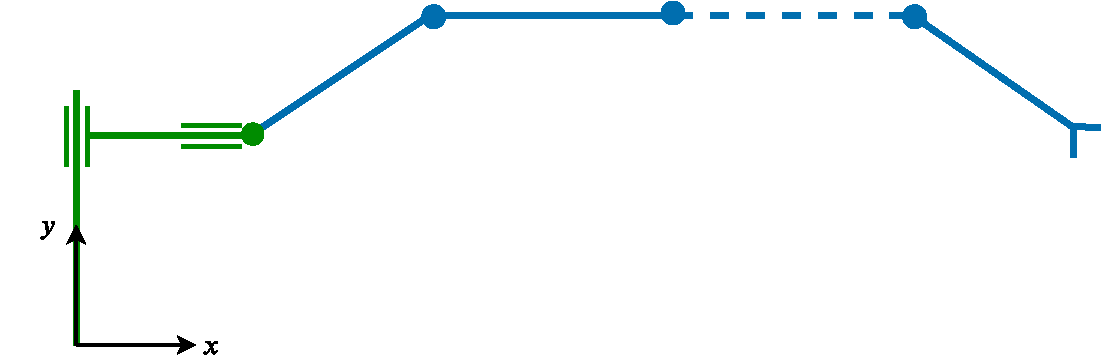
\includegraphics[width=0.9\textwidth]{figures/modelspecs/superbasicsnake.pdf}
    \caption{Model of snake robot with $n$ links}
    \label{fig:2_kin}
\end{figure}

%----------------------------------------------------------------------------------
%----------------------------------------------------------------------------------

\subsubsection{The environment}
The environment is the (x,y)-plane in Figure \ref{fig:2_kin}, and consists of nothing but the robot and the obstacles.

%----------------------------------------------------------------------------------
%----------------------------------------------------------------------------------


\subsubsection{The obstacles}

The obstacles are modeled as rigid points in the plane and any contact with them is considered a point contact. Figure \ref{fig:2_kin_obst} shows three obstacles in contact with a snake robot.

\begin{figure}[h!]
    \centering
    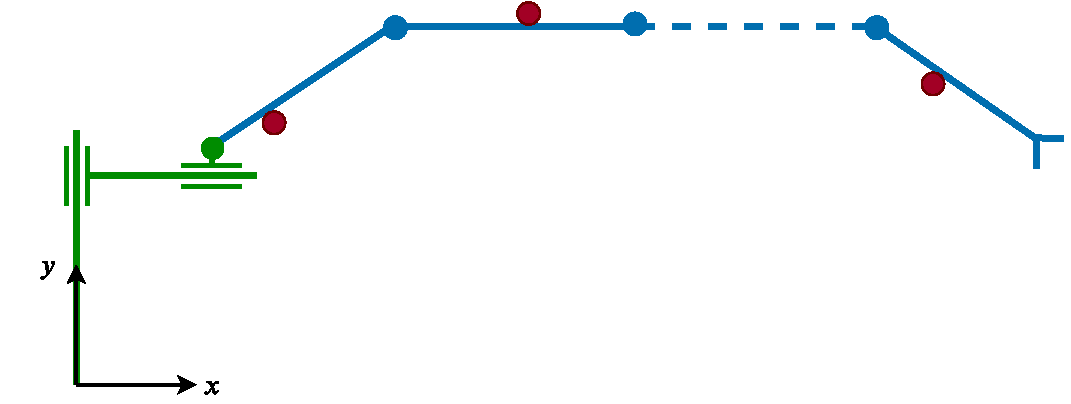
\includegraphics[width=0.9\textwidth]{figures/modelspecs/superbasicsnakenobstacles.pdf}
    \caption{Model of snake robot and obstacles}
    \label{fig:2_kin_obst}
\end{figure}








%\begin{itemize}
 %   \item Theoretical base
 %   \begin{itemize}
 %       \item A summary of the most significant snake robot locomotion strategies and a discussion of HPFC in light of these locomotion strategies
 %       \item Description of the snake robot specific kinematics and dynamics, with a focus on constrained snake robots
 %   \end{itemize}
 %   
 %   \item Dynamic HPFC for snake robots
 %   \begin{itemize}
 %      \item A thorough mathematical derivation of the dynamic HPFC for snake robots
 %       \item Modifications for increased control performance
 %       \item A discussion of ideal snake robot and obstacle configurations for general dynamic HPFC and for OAL
 %       \item An analysis of the benefits and limitations with special regard to snake robots vs. robot manipulators
  %      \item An analysis of the exploitation of the position and force spaces for propulsion
   %     \item A description of further requirements for the implementation of HOAL and dynamic HPFC on snake robots 
    %\end{itemize}
    %
    %\item Simulations
    %\begin{itemize}
    %    \item A description of the structure of the chosen simulator and comparison to corresponding simulators
    %    \item An evaluation of the validity of the simulators physics engine
    %    \item Implementation of the adapted dynamic HPFC method in the simulator
    %    \item An evaluation of the method through simulation experiments
    %\end{itemize}
%
%\end{itemize}


\section{Report structure}

It is assumed that the reader is familiar with basic robotics and control theory. A more thorough explanation of the topics can be found in \cite{lynch2017modern}, \cite{lynch2017modernCompTorque}, \cite{waldron2016kinematics}, \cite{liljeback2012snake}.

To begin with, the report introduces a set of different terrestrial snake robot locomotion strategies in Chapter \ref{chapter:theory}. This chapter also covers the required mathematical background theory for understanding the dynamical HPFC method. The dynamic HPFC method is then thoroughly explained in Chapter \ref{ch:hpfc}. All related considerations and limitations are also provided here. Chapter \ref{chapter:simulator} explains the structure of the chosen simulator and how it is used for the simulated experiments, which are presented in Chapter \ref{ch:results}. The results from the experiments and general analysis of the dynamic HPFC method on snake robots are discussed in Chapter \ref{ch:discussion}. Lastly, Chapter \ref{ch:conclusion} concludes the work and Chapter \ref{ch:future} proposes some ideas for future research and possible improvements based on the challenges encountered in this project.